\author{Tavo Annus, Timo Loomets, Mattias Kitsing}
\title{%
   Localization recap \\
  \large Team SCITOS-02}
\date{\today}

%%%%%%%%%%%%%%%%%
% Configuration %
%%%%%%%%%%%%%%%%%

\documentclass[12pt, a4paper, onecolumn]{article}
\usepackage{xurl}
\usepackage[super,comma,sort&compress]{natbib}
\usepackage{graphicx}
\usepackage{abstract}
\usepackage{enumitem}
\usepackage{lipsum,booktabs}
\renewcommand{\abstractnamefont}{\normalfont\bfseries}
\renewcommand{\abstracttextfont}{\normalfont\small\itshape}
\usepackage{lipsum}

% Any configuration that should be done before the end of the preamble:
\usepackage{hyperref}
\hypersetup{colorlinks=true, urlcolor=blue, linkcolor=black, citecolor=blue}
\setlength{\belowcaptionskip}{-10pt}
\pagenumbering{gobble}
%\pagenumbering{arabic}
\renewcommand\thesection{}
\setlength{\parindent}{0em}
\setlength{\parskip}{0,8em}
\addtolength{\topmargin}{-60pt}
\addtolength{\textheight}{120pt}
\linespread{1.25}

\begin{document}
\maketitle
%%%%%%%%%%%
% Article %
%%%%%%%%%%%

% Intro %
\section{The good}
Our EKF performed significantly better than the naive odometry implementation, especially considering the intergrated error.
For naive implementation the error keeps accumulating but EKF managed to keep it somewhat low as shown in the figure~\ref{fig:err_x} or~\ref{fig:ekf_good}.

\begin{figure}[h!]
  \begin{center}
    \includegraphics[width=0.95\textwidth]{./fig/ekf_errors/x.png}
  \end{center}
  \caption{EKF x error}
  \label{fig:err_x}
\end{figure}

\begin{figure}[h!]
  \begin{center}
    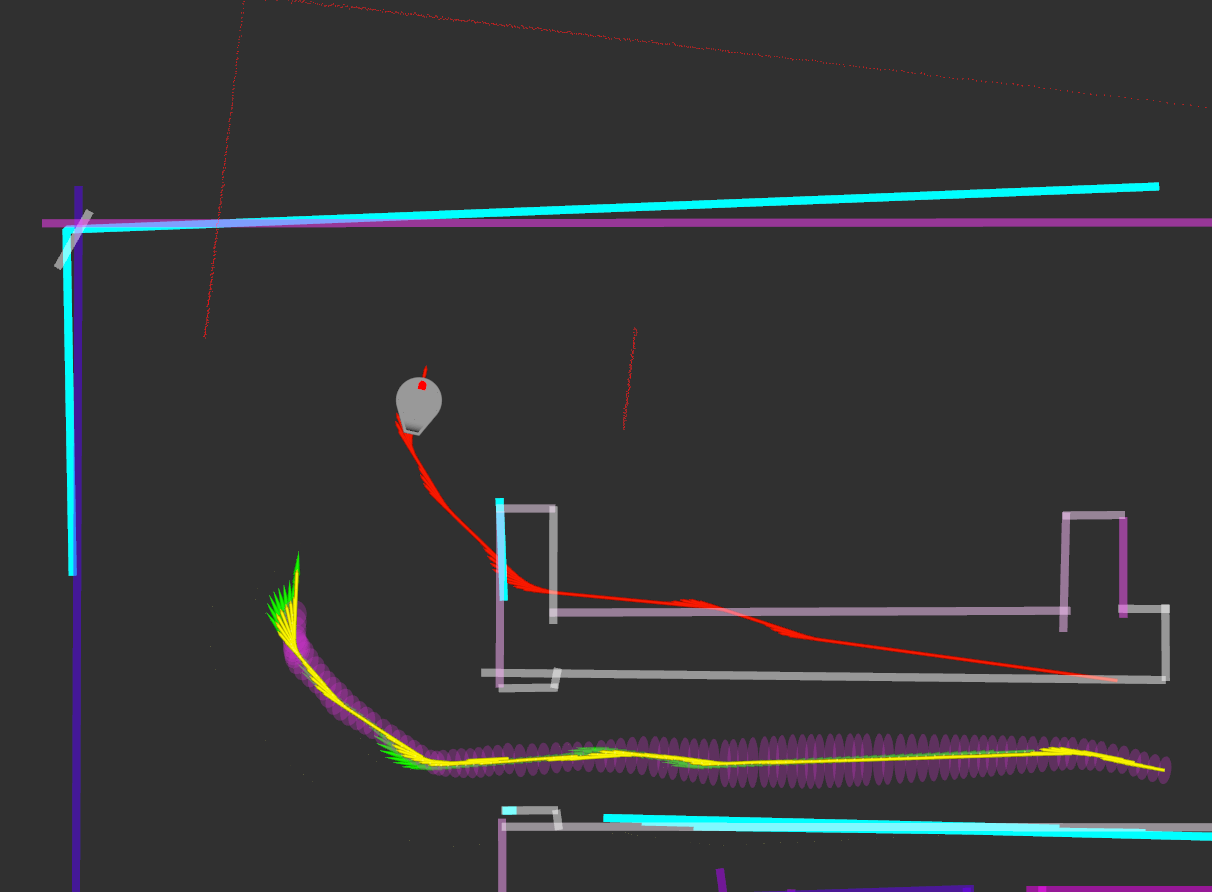
\includegraphics[width=0.95\textwidth]{./fig/ekf_good.png}
  \end{center}
  \caption{EKF performing good}
  \label{fig:ekf_good}
\end{figure}


\newpage
\section{The bad}
However the EKF didn't give us much improvement when there were lack of features, for example too long walls as we considered only line endings as features.
The uncertanity kept increasing in that case as shown in the figure~\ref{fig:err_y}.
\begin{figure}[h!]
  \begin{center}
    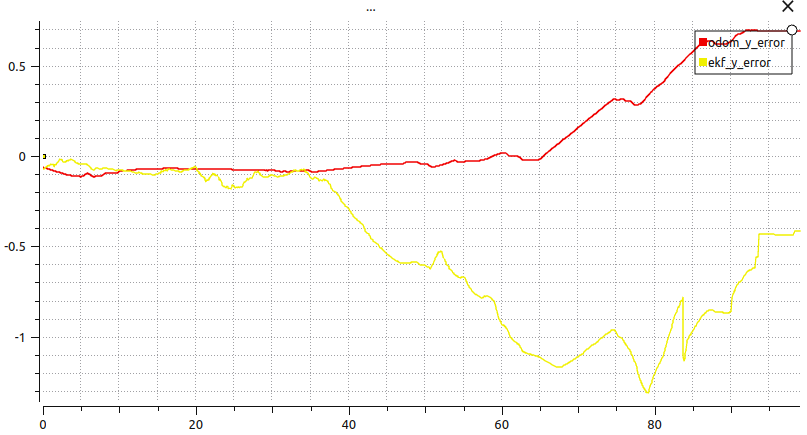
\includegraphics[width=0.95\textwidth]{./fig/ekf_errors/y.png}
  \end{center}
  \caption{EKF y error}
  \label{fig:err_y}
\end{figure}
Note that both the graph for x and y come from the same run meaning that sometimes (depending on feature locations) the algorithm managed
to zero in on one axis but not on the other.

Sometimes the EKF algorithm managed to recover quite well from these kind of situations, but if the error accumulated to be too big it failed.
\begin{figure}[h!]
  \begin{center}
    \includegraphics[width=0.95\textwidth]{./fig/ekf_recovery.png}
  \end{center}
  \caption{EKF recovering from some error}
  \label{fig:ekf_recovery}
\end{figure}


\newpage
\section{The ugly}

There was also quite a lot of problems with incorrectly mapped features that caused localization to jump.
These were common to corners of the map where some double lines existed.
We added some sanity checks to avoid these jumps as they completely broke the localization in some cases, but the heuristics anly helped to some extent.

Some of these jumps in yaw can be seen in the figure~\ref{fig:rmse}.

\begin{figure}[h!]
  \begin{center}
    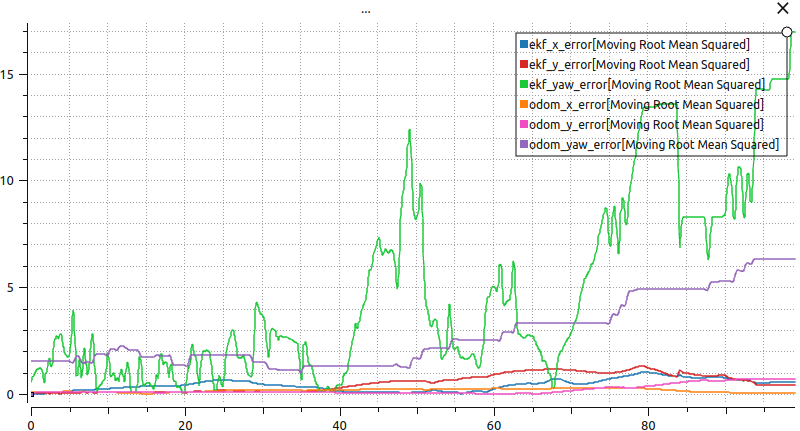
\includegraphics[width=0.95\textwidth]{./fig/ekf_errors/RMS.png}
  \end{center}
  \caption{RMSE for EKF and odometry}
  \label{fig:rmse}
\end{figure}

\newpage
\section{Overall}
Overall EKF improved the localization a lot.
It made possible to drive for a lot longer, basically it failed in some bad situations but not due to slowly accumulating error.
We are planning to switch to motion model that uses odometry instead of velocity commands to hopefully have slightly better estimates.
If we manage to build wrapper that deals with kidnapping problem, it would likely also help to recover from places where multiple features get incorrectly
mapped and the algorithm breaks.
However that is a workaround we are not going to start building (at least right away).


\end{document}

